% !TEX root = ../om_ts_01.tex

\begin{frame} % название фрагмента

\videotitle{Алгоритм STL}

\end{frame}



\begin{frame}{Алгоритм STL: план}
  \begin{itemize}[<+->]
    \item Локальная регрессия.
    \item Внешний цикл STL.
    \item Внутренний цикл STL.
    \item Параметры STL.
  \end{itemize}

\end{frame}


\begin{frame}{STL}

  \alert{STL} — Seasonal Trend decompositon with Loess.
  
  STL — разложение на сезонность и тренд с использованием LOESS.
  
  \pause
  
  \alert{LOESS} — LOcal regrESSion.
  
  LOESS — локальная линейная регрессия. 
  
\end{frame}


\begin{frame}{STL как чёрный ящик}

\alert{На входе:}

Ряд $Y_t$.

Параметры алгоритма $n_p$, $n_i$, $n_o$, $n_l$, $n_s$, $n_t$.

\pause
\alert{На выходе:}

Разложение $Y_t = T_t + S_t + R_t$.

\pause

Чёрный ящик \alert{долго} настраивали. 

\end{frame}


\begin{frame}{STL: результат}

  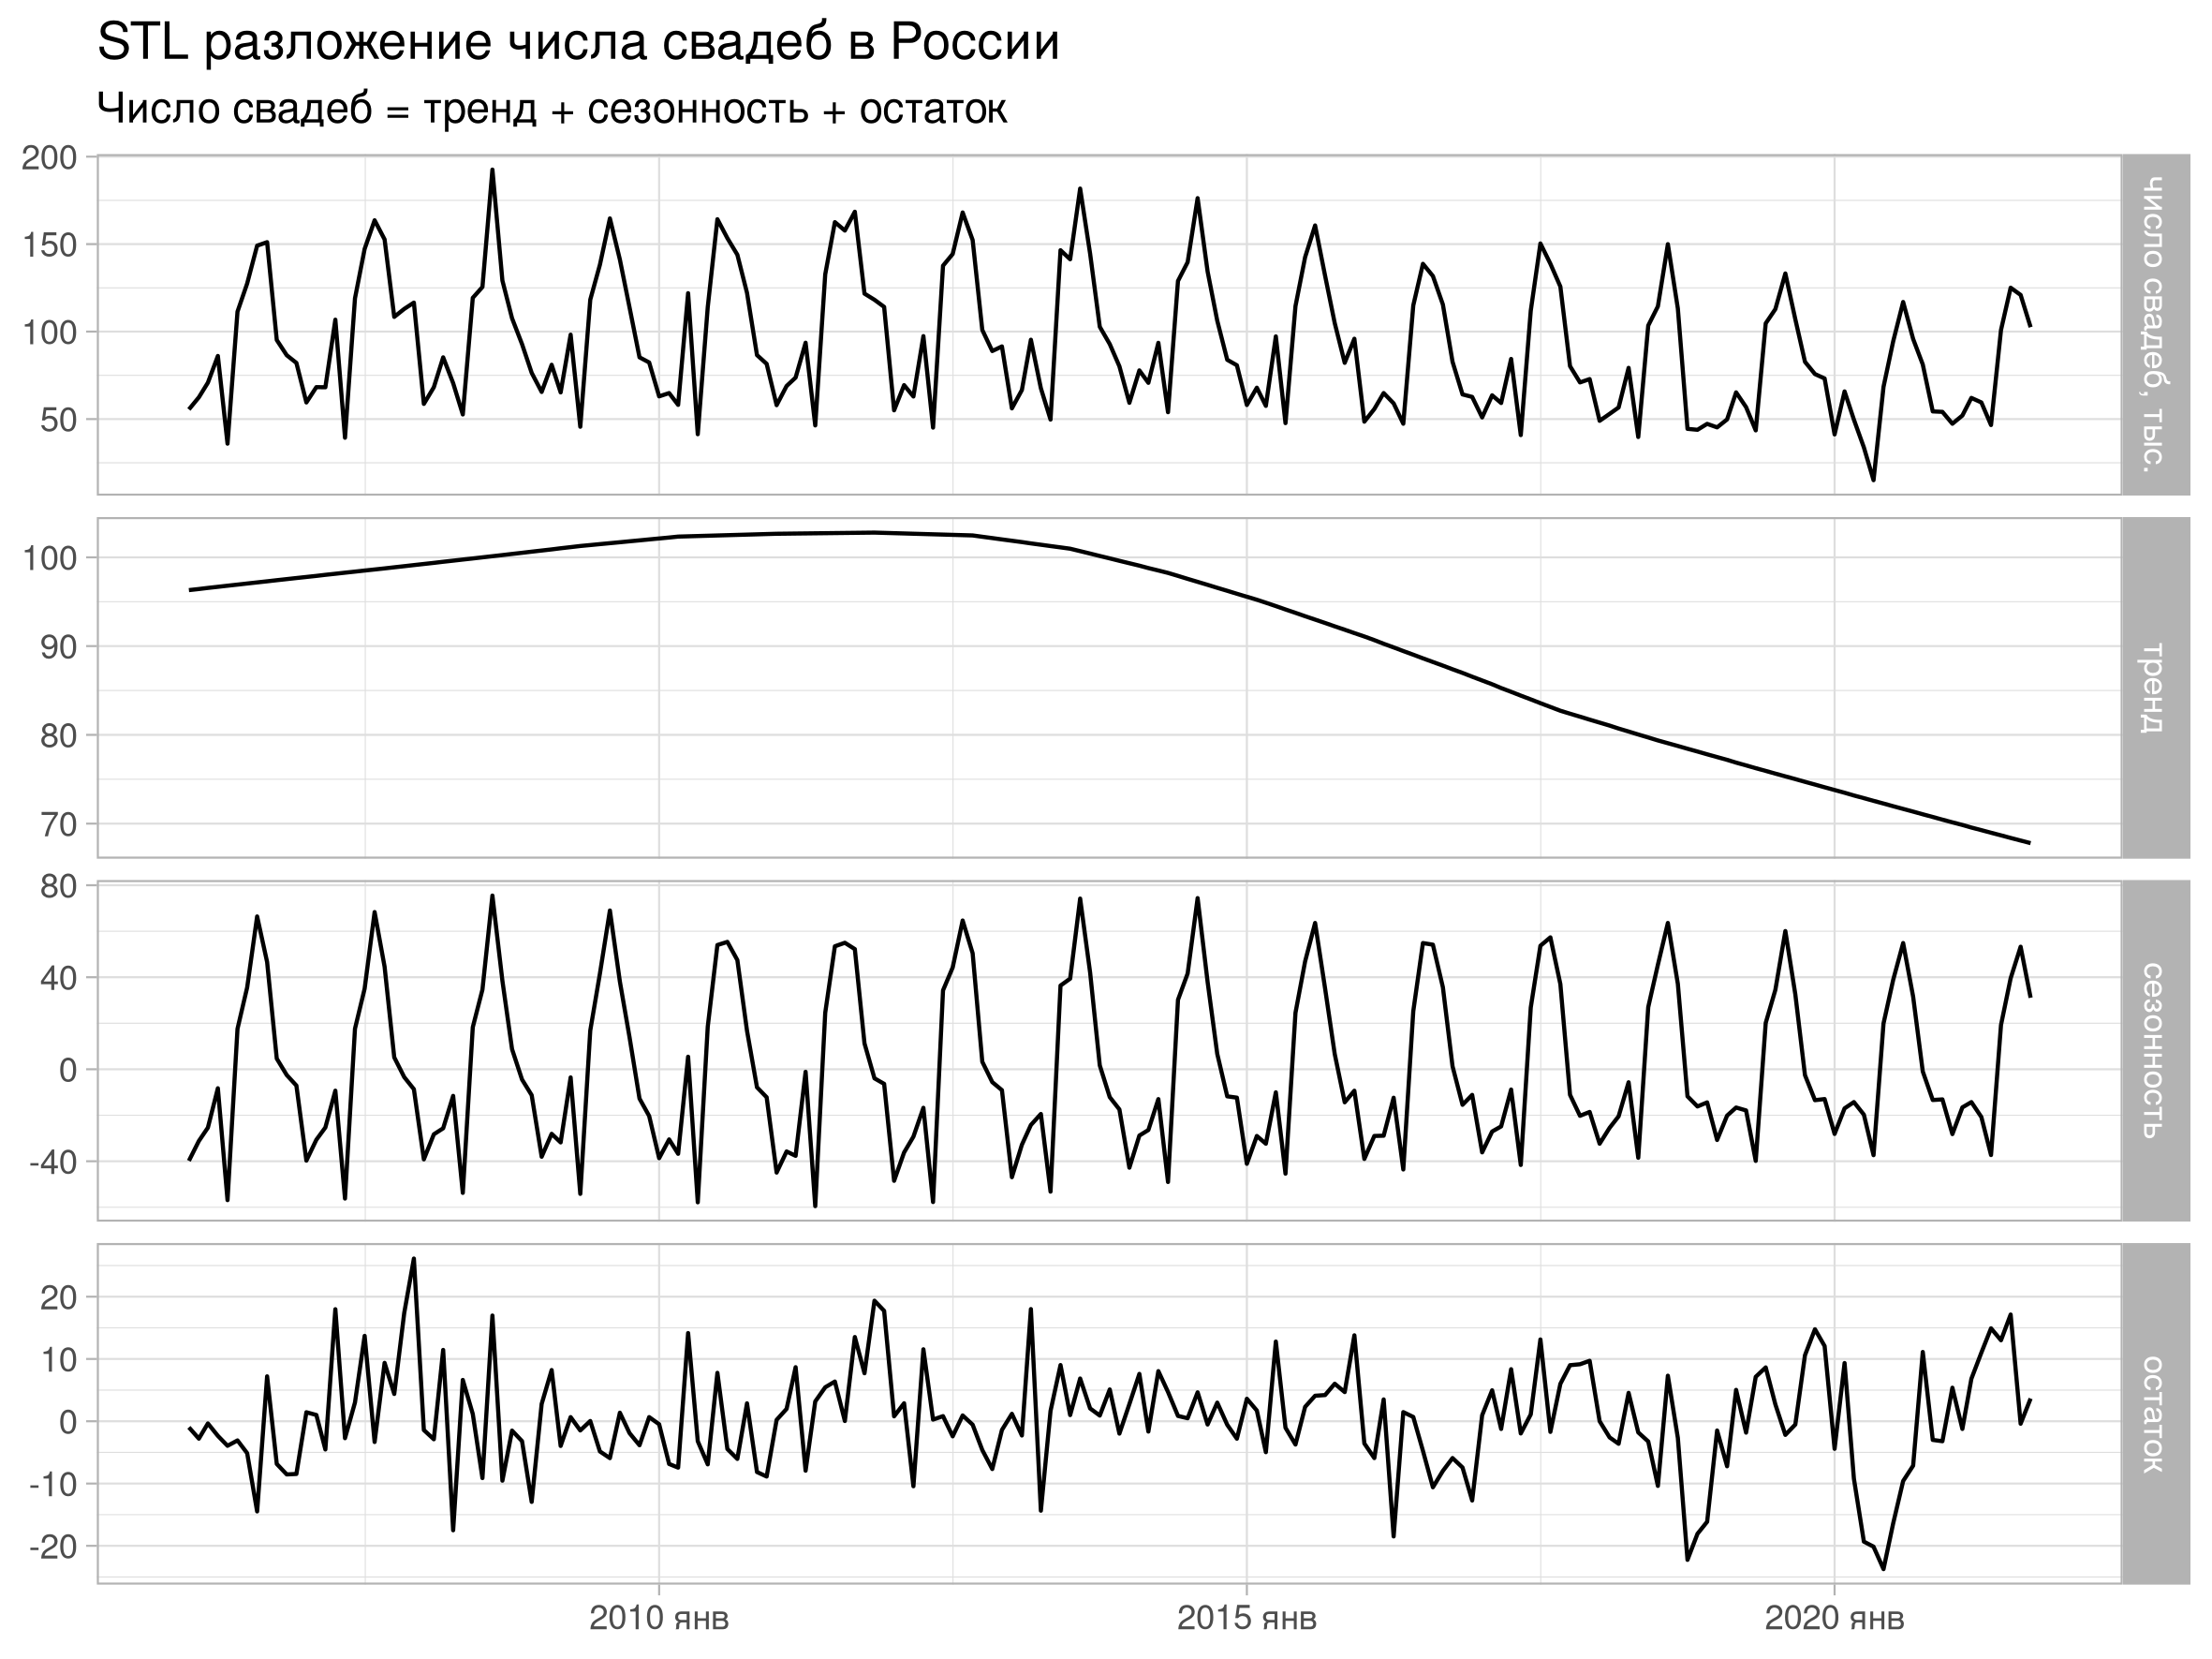
\includegraphics[width=\textwidth]{pictures/om_ts_01-074.png}


\end{frame}

\begin{frame}{LOESS}

\begin{itemize}
  \item Хотим построить прогноз для точки $x$.
  \item Находим \alert{локальные оценки} $\hat\beta_1(x)$, $\hat\beta_2(x)$. 
  \[
      \min \sum_i \alert{K_h(x_i - x)} (y_i - \hat\beta_1 - \hat\beta_2 x_i)^2
  \]
  \item Прогнозируем:
  \[
  \hat y = \hat\beta_1(x) + \hat\beta_2(x) x.  
  \] 
\end{itemize}

\pause
\alert{Ядерная функция}
\begin{itemize}
  \item Функция $K_h(x_i - x)$ убывает с увеличением расстояния $|x_i - x|$;
  \item Параметр $h$ отвечает за ширину окна сглаживания. 
\end{itemize}

\pause
Например, $h$ — количество точек $x_i$ рядом с $x$, которые мы учитываем.

\end{frame}

\begin{frame}{Нюансы локальной регрессии}

  \begin{itemize}
    \item Выбор \alert{степени полинома}.
    \[
      \min \sum_i \alert{K_h(x_i - x)} (y_i - \hat\beta_1 - \hat\beta_2 x_i - \hat\beta_3 x_i^2)^2
    \]  
    \item Выбор \alert{ядерной} функции.
    \[
      K_h(d) = \frac{1}{\sqrt{2\pi}h} \exp(- d^2/2h^2)
    \]
    \item Выбор \alert{ширины окна} $h$.

\end{itemize}

\end{frame}

\begin{frame}{STL с высоты птичьего полёта}

Цель: разложение $Y_t = T_t + S_t + R_t$.

Алгоритм содержит два цикла: \alert{внешний} и \alert{внутренний}.

\begin{enumerate}[<+->]

  \item Инициализируем $T_t = 0$, $R_t = 0$.
  
  \alert{Внешний} цикл:

  \item Посчитаем вес каждого наблюдения, $\rho_t$. 

  На первом проходе $\rho_t = 1$ у каждого наблюдения. 

  На последующих проходах $\rho_t$ отрицательно зависит от свежей величины $R_t$.

  \item Обновим текущее разложение $Y_t = T_t + S_t + R_t$ с учётом весов $\rho_t$.
\end{enumerate}

\end{frame}



\begin{frame}{STL: внутренний цикл}

  Цель: обновить разложение $Y_t = T_t + S_t + R_t$.
  
  \begin{enumerate}[<+->]
  
    \item[1.] Удалим из ряда ранее посчитанный тренд:
    \[
      Y_t^{det} = Y_t - T_t.
    \]
    
    \item[2.] Разобъём детрендированный ряд на 12 подрядов. 
    
    \item[3.] Сгладим каждый подряд по отдельности с помощью LOESS:
    \[
    C^{jan} = LOESS_{\rho}(Y^{det}_{jan}), C^{feb} = LOESS_{\rho}(Y^{det}_{feb}), \ldots
    \]

    \item[4.] Выделяем низкочастотную составляющую (дважды скользящее среднее + LOESS):
    \[
    L_t = LOESS(MA(MA(C_t)))
    \]    
    \item[5-6.] Получаем новые $S_t^{new}$ и $T_t^{new}$.
  \end{enumerate}
  
  
  \end{frame}
  


  \begin{frame}{STL: внутренний цикл}
    
    \begin{enumerate}[<+->]
    
      \item[1-3.] Удалим из ряда ранее посчитанный тренд, разобъём на подряды и 
      сгладим каждый подряд с помощью LOESS. 
      
      \item[4.] Выделяем низкочастотную составляющую.
      \item[5.] Удаляем низкочастотную составляющую, получаем \alert{новую} сезонную компоненту:
      \[
      S_t^{new} = C_t - L_t.  
      \]
      \item[6.] Удаляем новую сезонность из исходного ряда и сглаживаем с помощью LOESS:
      \[
      T_t^{new} = LOESS_{\rho}(Y_t - S_t^{new}).
      \]
      
    \end{enumerate}
    
    
    \end{frame}
    
  
    \begin{frame}

      \begin{center}
        Уф!
      \end{center}

    \end{frame}
  

\begin{frame}{Параметры STL}

  \begin{itemize}[<+->]
    \item $n_p$ — периодичность сезонности, например, $n_p=12$.
    \item $n_o$ — число проходов внешнего цикла. 
    
    Чем больше число $n_o$, тем слабее влияние выбросов.

    Значение $n_o = 1$ часто достаточно.
    \item $n_i$ — число проходов внутреннего цикла. 

    Значение $n_i = 2$ часто достаточно для достижения сходимости.
  \end{itemize}
    
\end{frame}

\begin{frame}{Параметры сглаживания STL}

\begin{itemize}[<+->]
\item $n_l$ — сила сглаживания низкочастотного фильтра. 

\item $n_s$ — сила сглаживания сезонных подрядов.
\item $n_t$ — сила сглаживания при выделении тренда на последнем шаге. 

\end{itemize}

\alert{Что настроить?}
\begin{enumerate}[<+->]
  \item Обязательно указать периодичность $n_p$.
  \item Возможно, поиграться с $n_s$.
\end{enumerate}

\end{frame}

\begin{frame}{STL: итоги}
  \begin{itemize}[<+->]
    \item LOESS — локальная регрессия.
    \item STL — хорошо проверенный временем алгоритм без модели.
    \item При желании можно поиграться с силами сглаживания.
  \end{itemize}

\end{frame}



